% Construction : a = (0, 0), b = (4,5 ; 1), c = (3 ; 3,2), et t = 0,6.
% Les points b' = a + t(b − a) et c' = a + t(c − a) portent la parallèle à (bc).
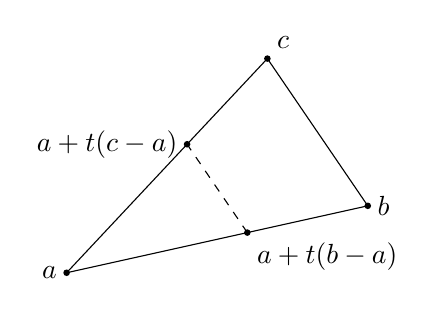
\begin{tikzpicture}[scale=0.85]
  \coordinate (a) at (0, 0);
  \coordinate (b) at (4.5, 1);
  \coordinate (c) at (3, 3.2);
  \coordinate (bp) at (2.7, 0.6);
  \coordinate (cp) at (1.8, 1.92);
  \draw (a) -- (b);
  \draw (a) -- (c);
  \draw (b) -- (c);
  \draw[dashed] (bp) -- (cp);
  \foreach \p in {a, b, c, bp, cp} \fill (\p) circle (1.4pt);
  \node[left] at (a) {$a$};
  \node[right] at (b) {$b$};
  \node[above right] at (c) {$c$};
  \node[below right] at (bp) {$a + t(b - a)$};
  \node[left] at (cp) {$a + t(c - a)$};
\end{tikzpicture}
